\begin{figure}
  \centering
  \begin{tabular}{c}
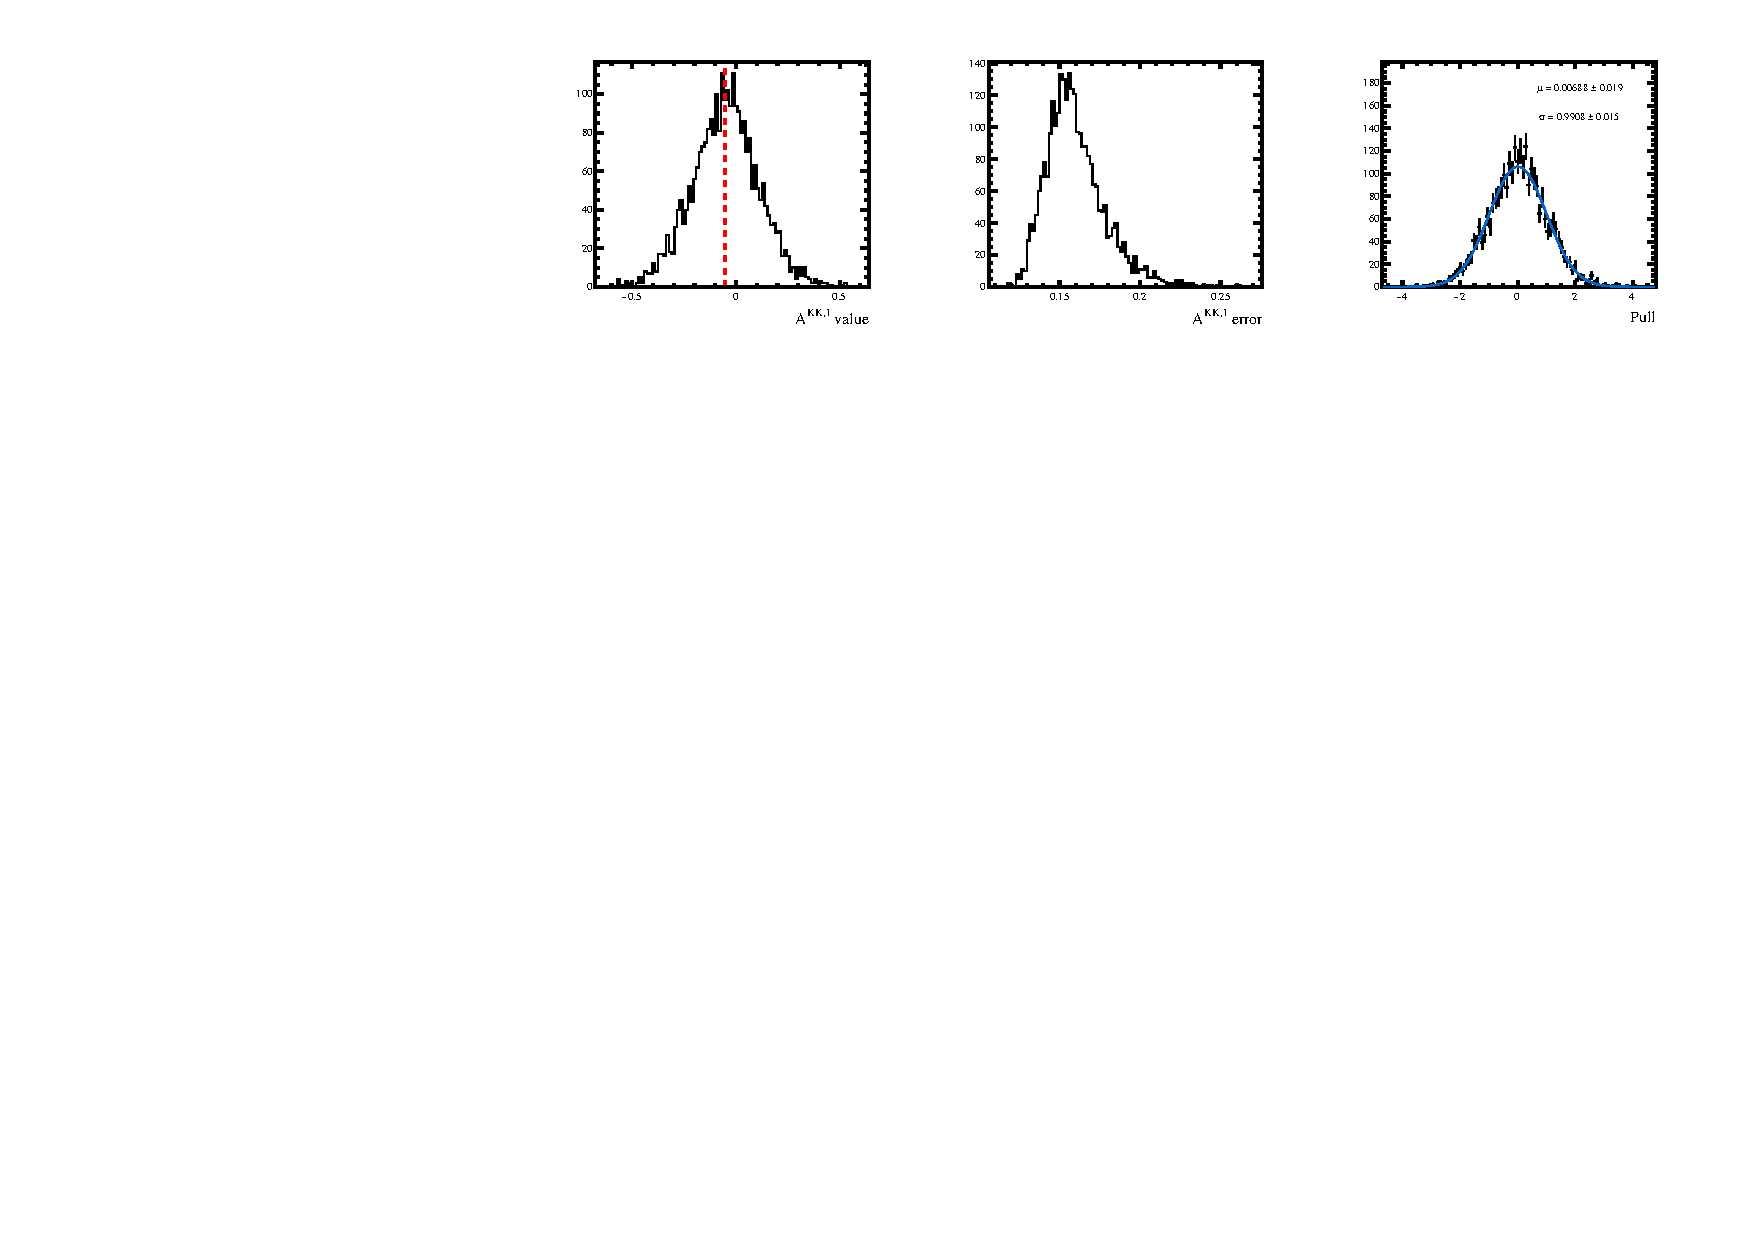
\includegraphics[width=0.7\textwidth]{ANA_resources/Plots/Data_fit/FitterBias//A_signal_KK_run1.pdf} \\
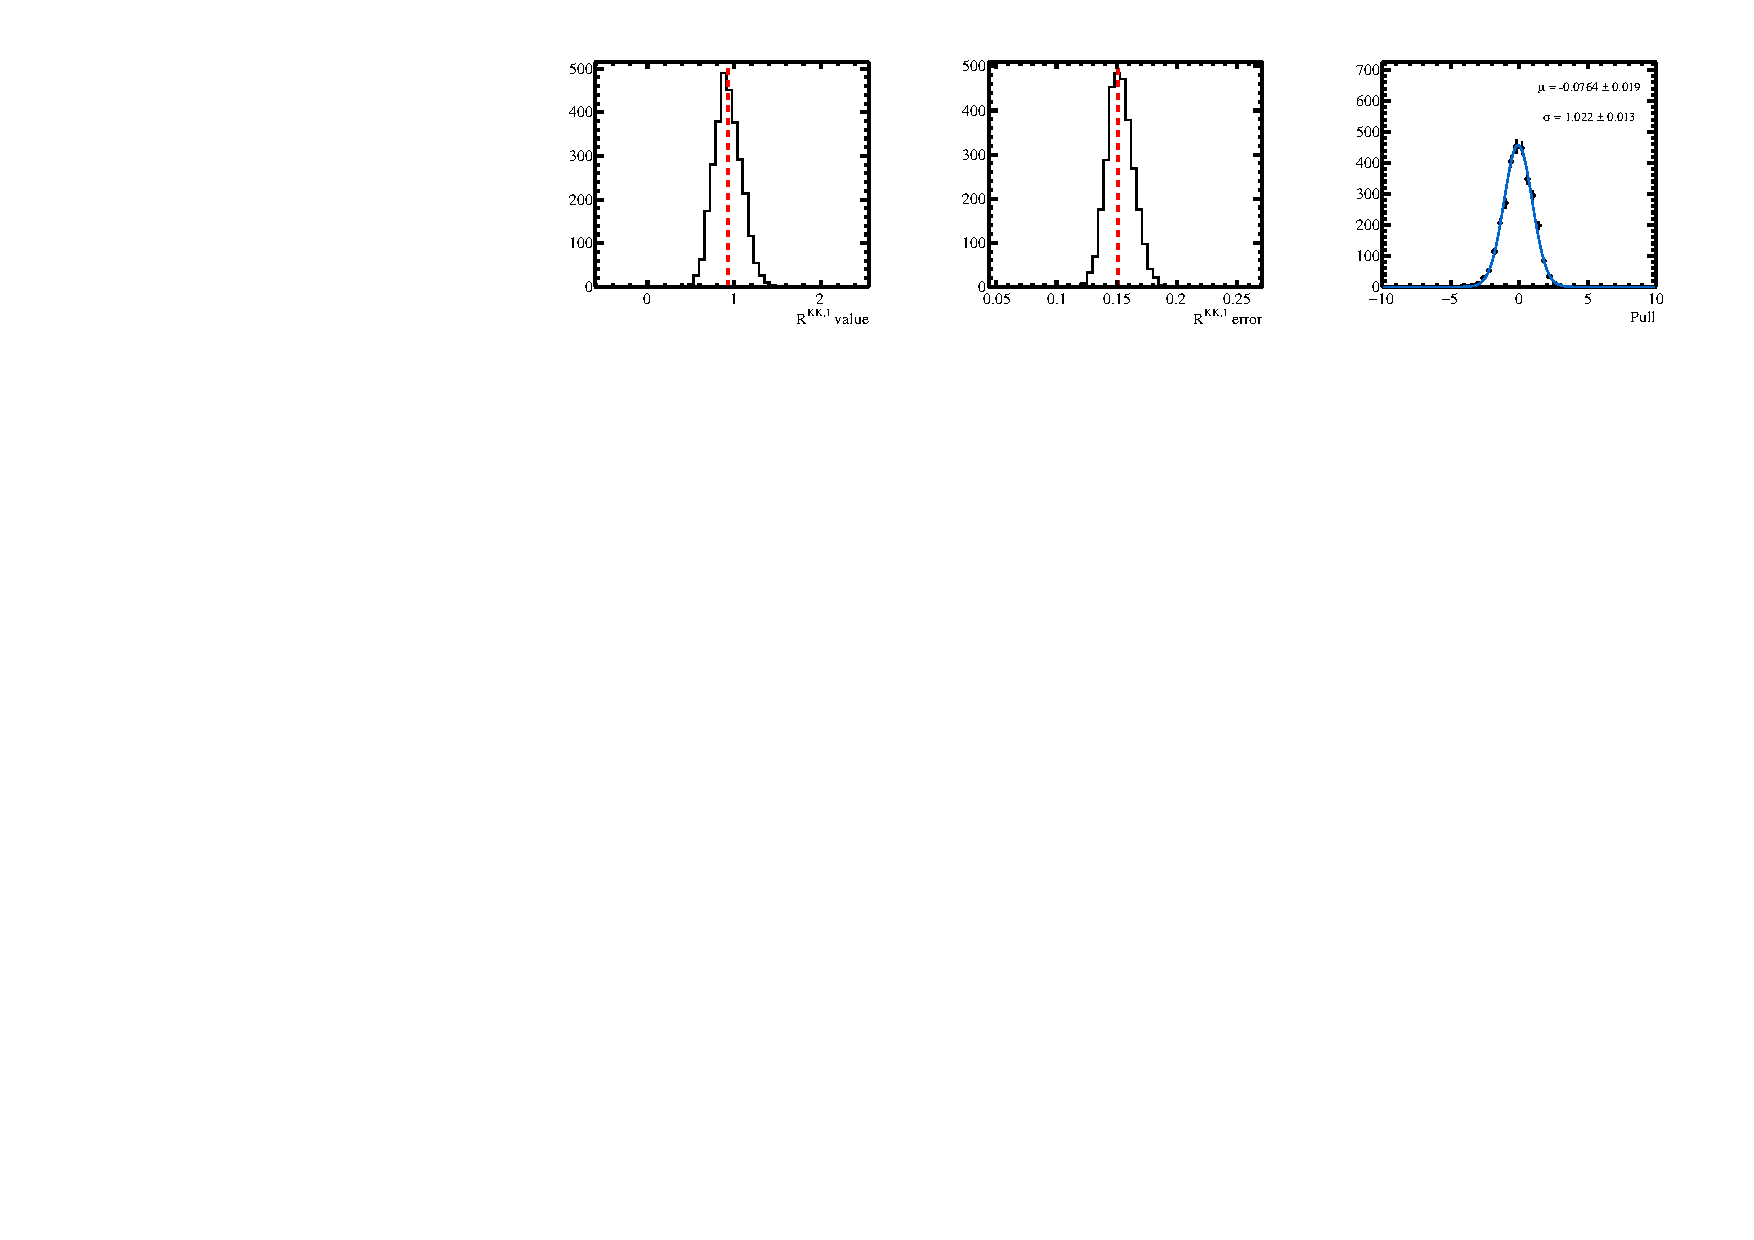
\includegraphics[width=0.7\textwidth]{ANA_resources/Plots/Data_fit/FitterBias//R_signal_KK_run1.pdf} \\
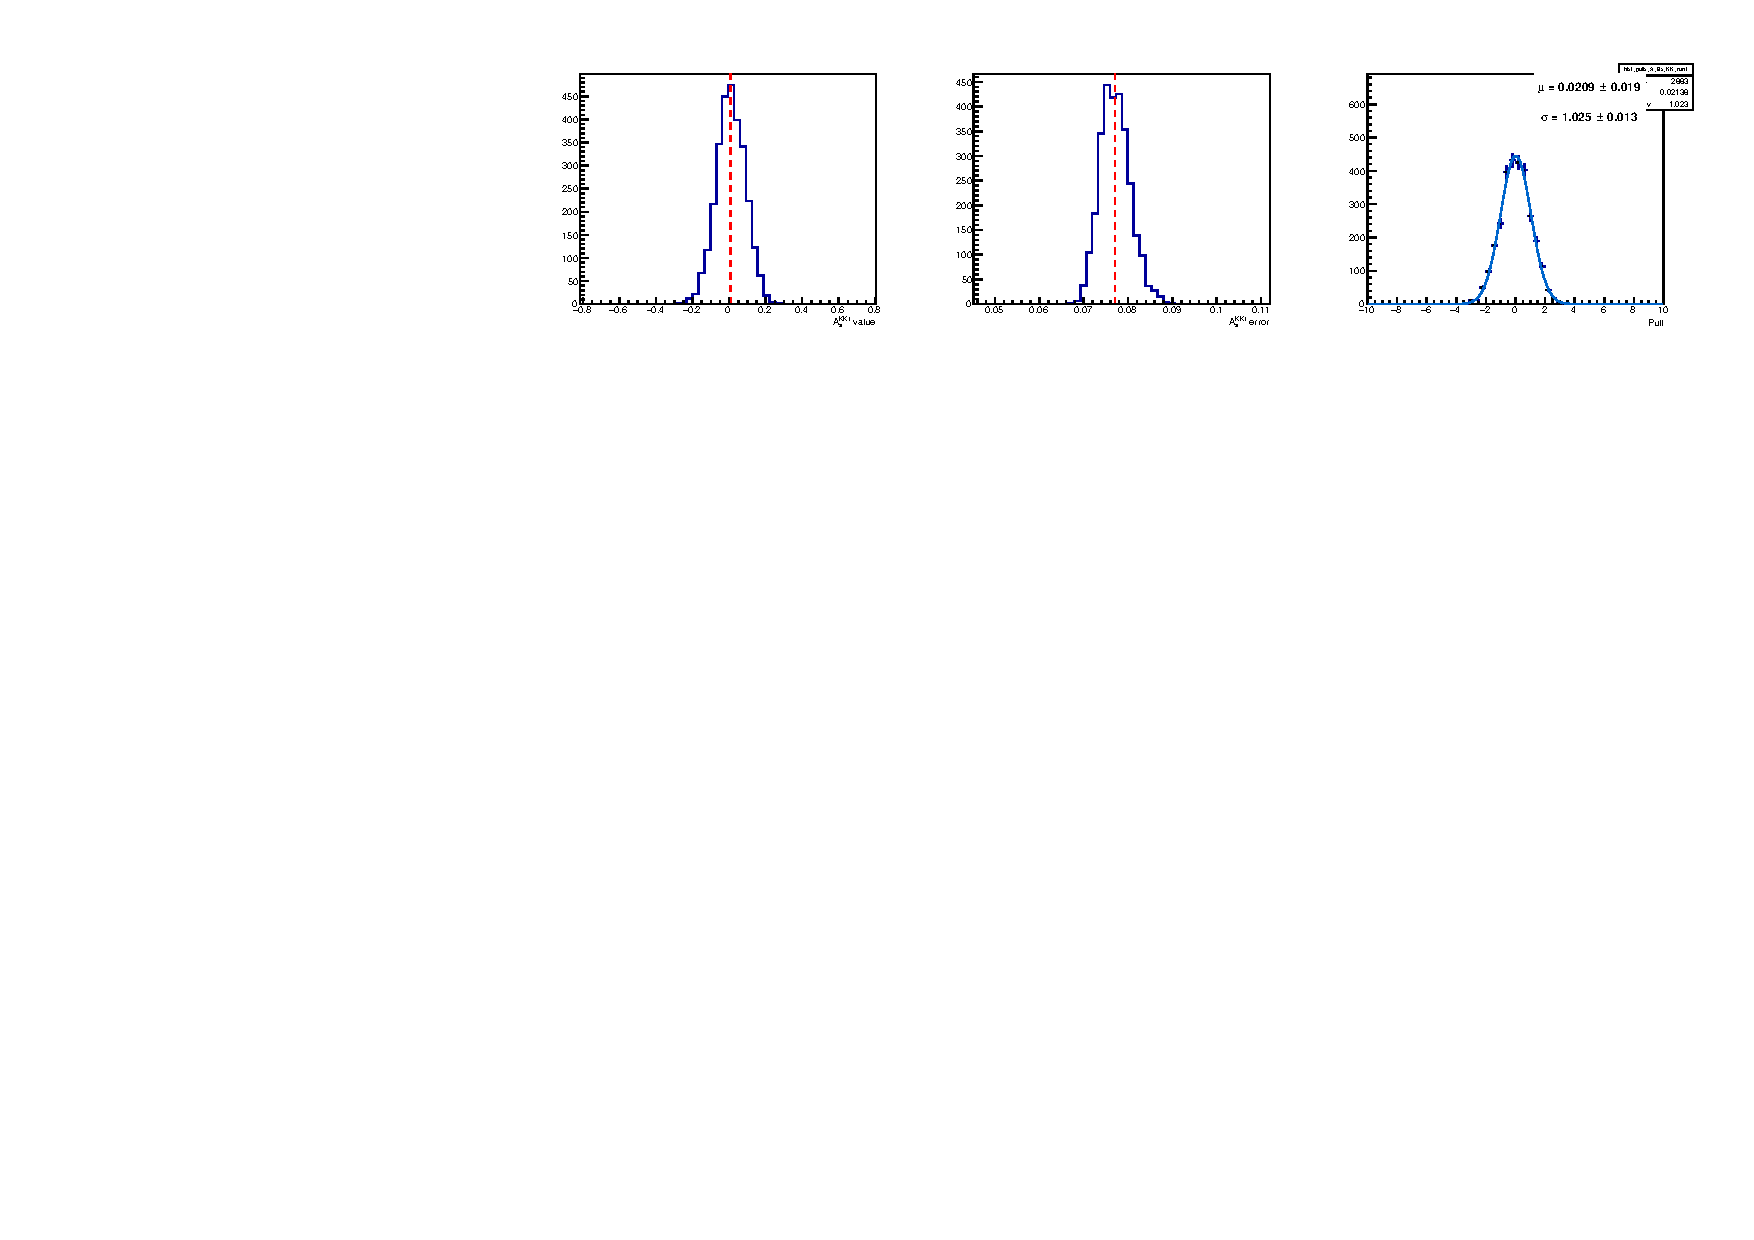
\includegraphics[width=0.7\textwidth]{ANA_resources/Plots/Data_fit/FitterBias//A_Bs_KK_run1.pdf} \\
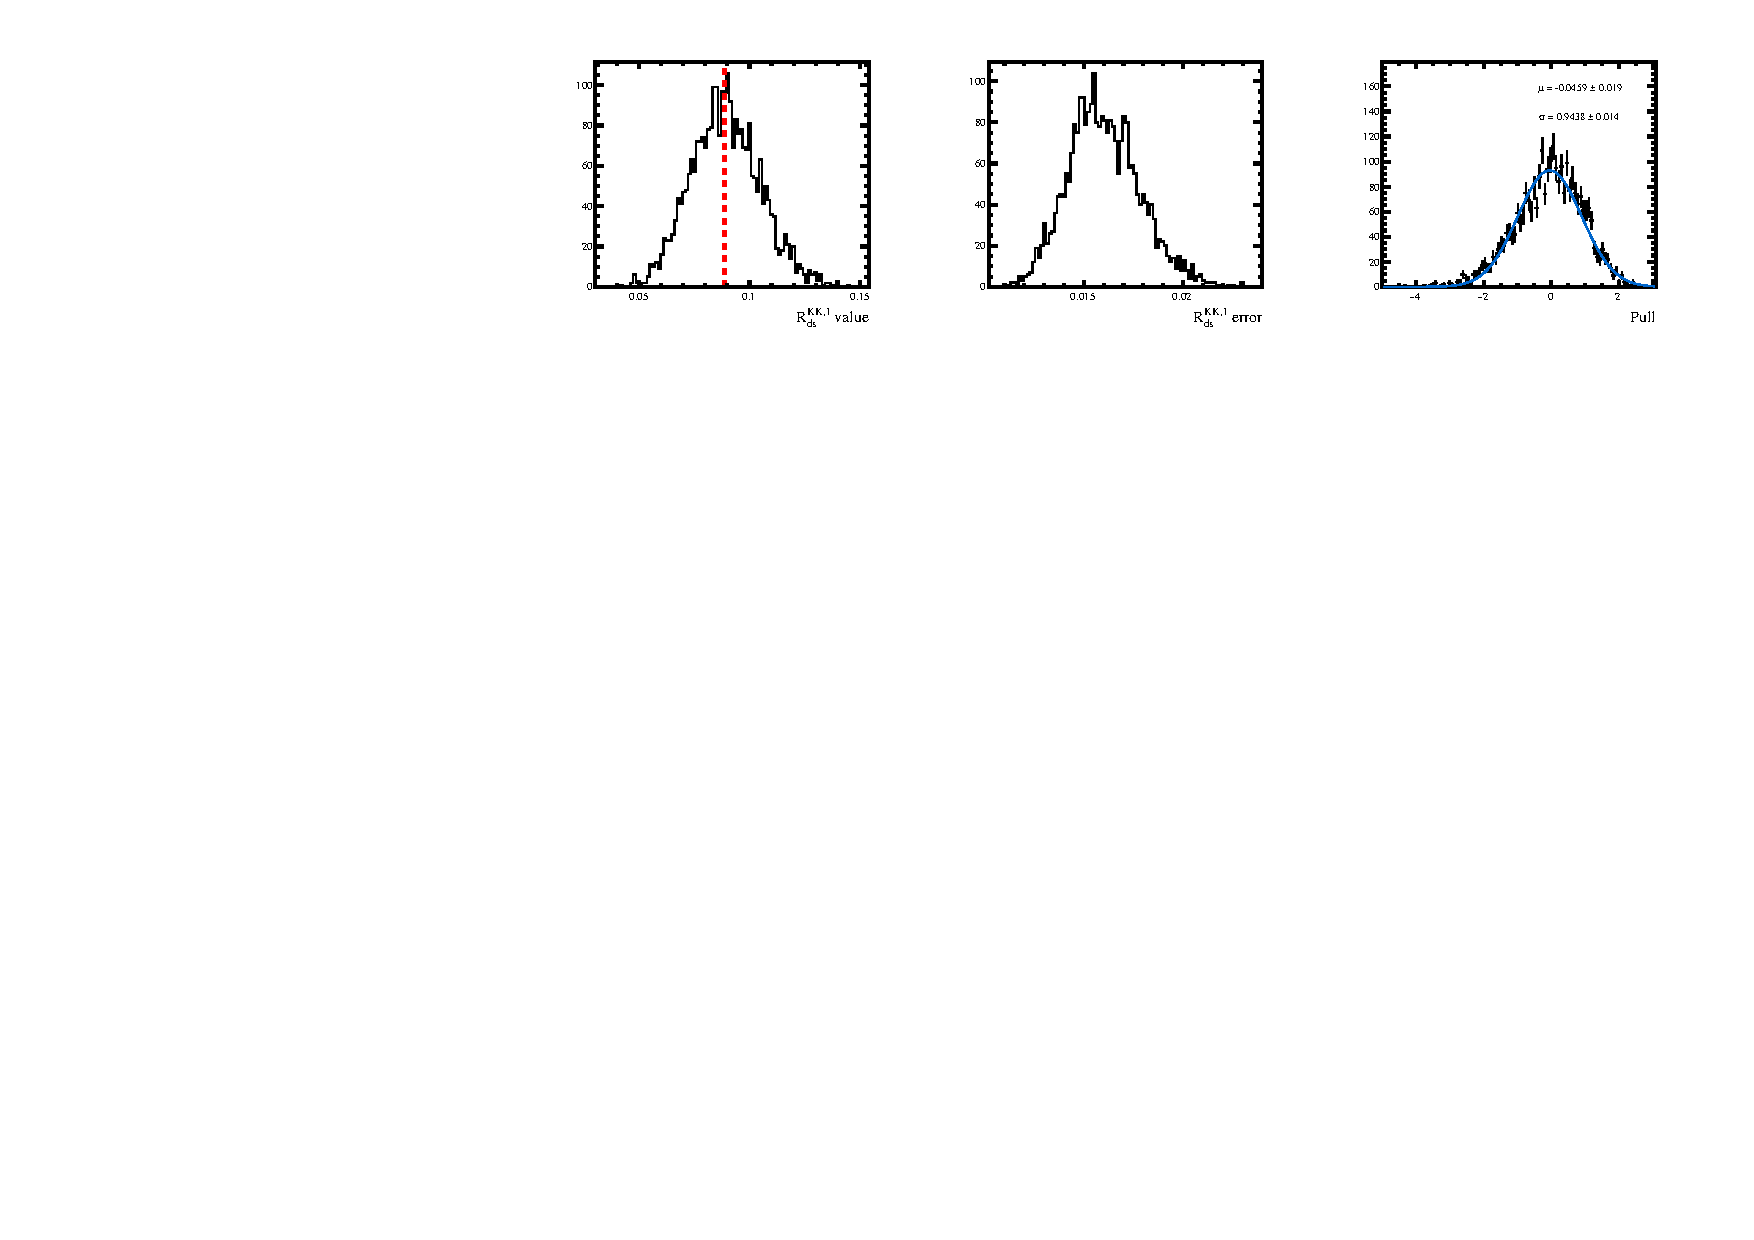
\includegraphics[width=0.7\textwidth]{ANA_resources/Plots/Data_fit/FitterBias//R_ds_KK_run1.pdf} \\
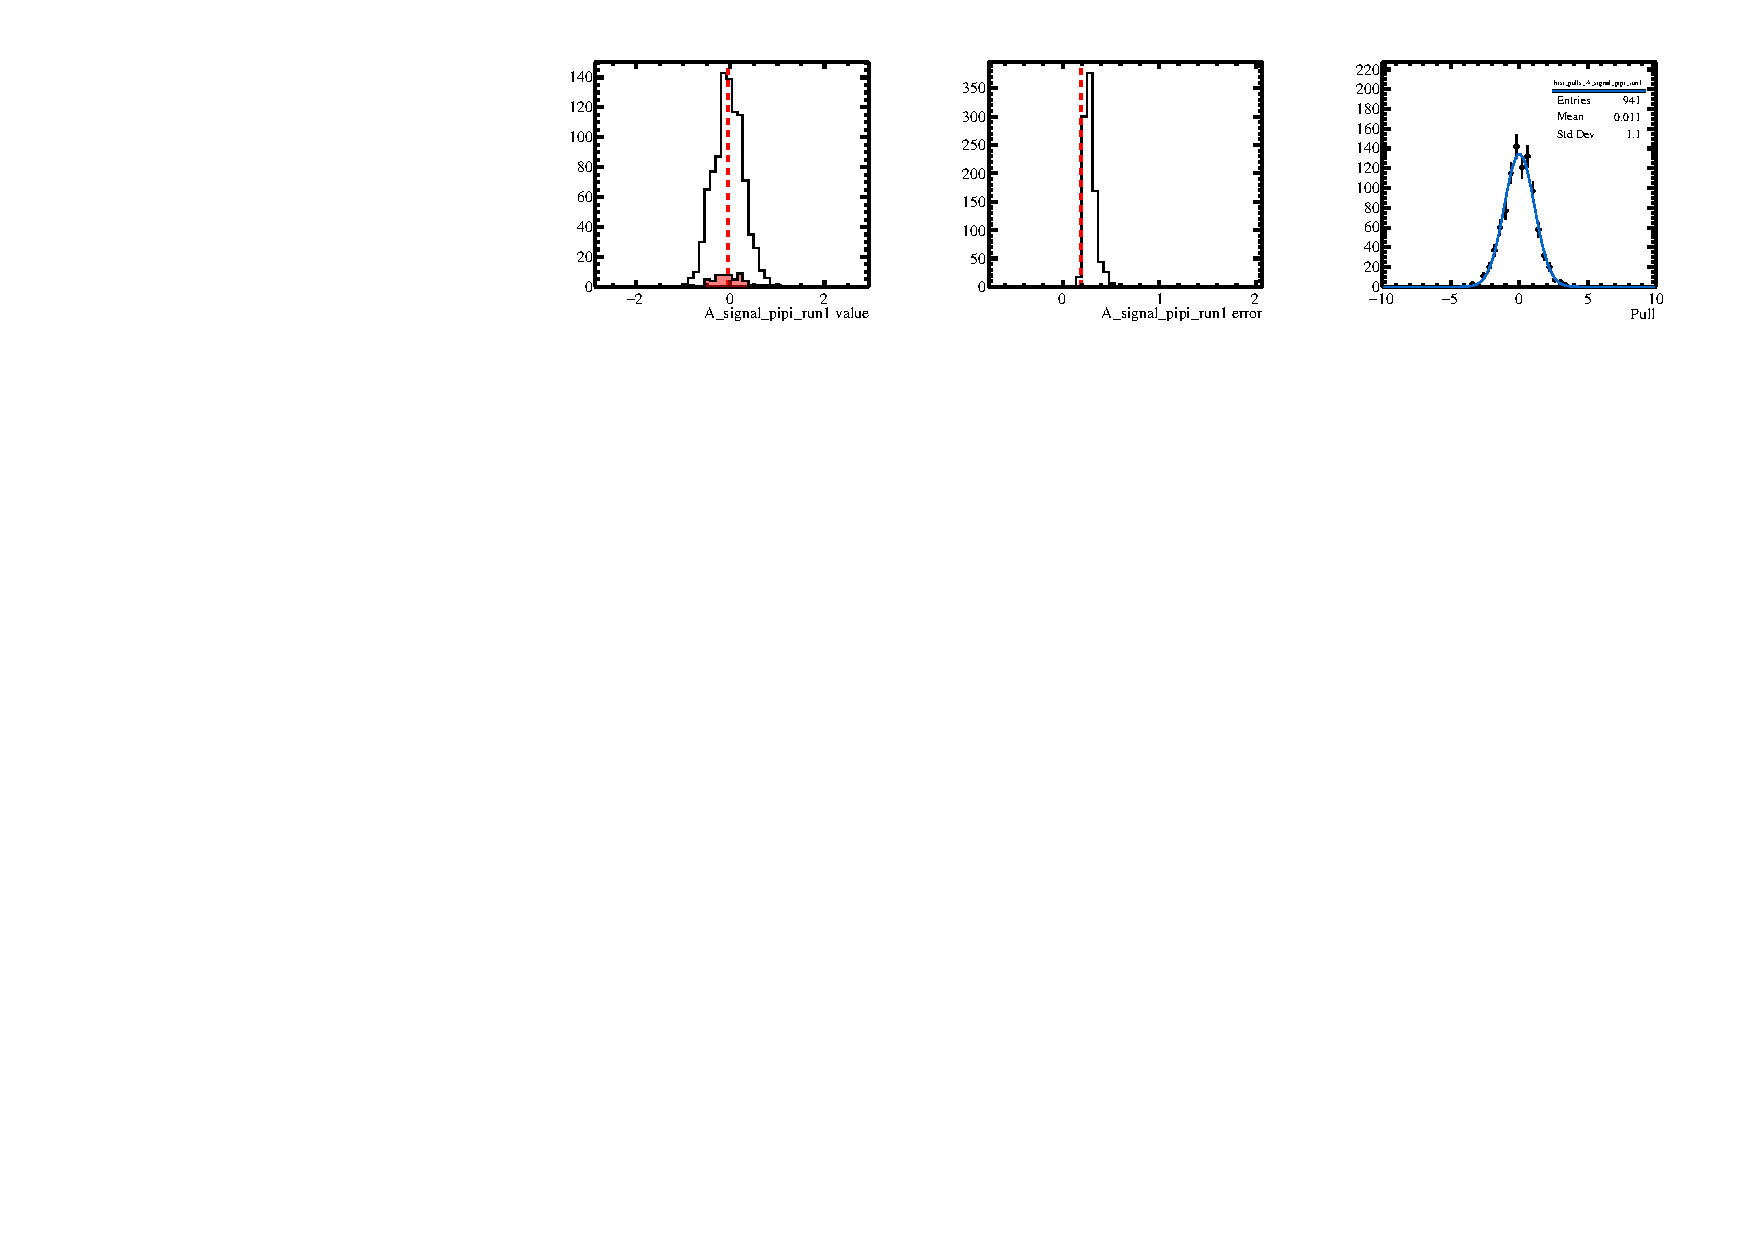
\includegraphics[width=0.7\textwidth]{ANA_resources/Plots/Data_fit/FitterBias//A_signal_pipi_run1.pdf} \\
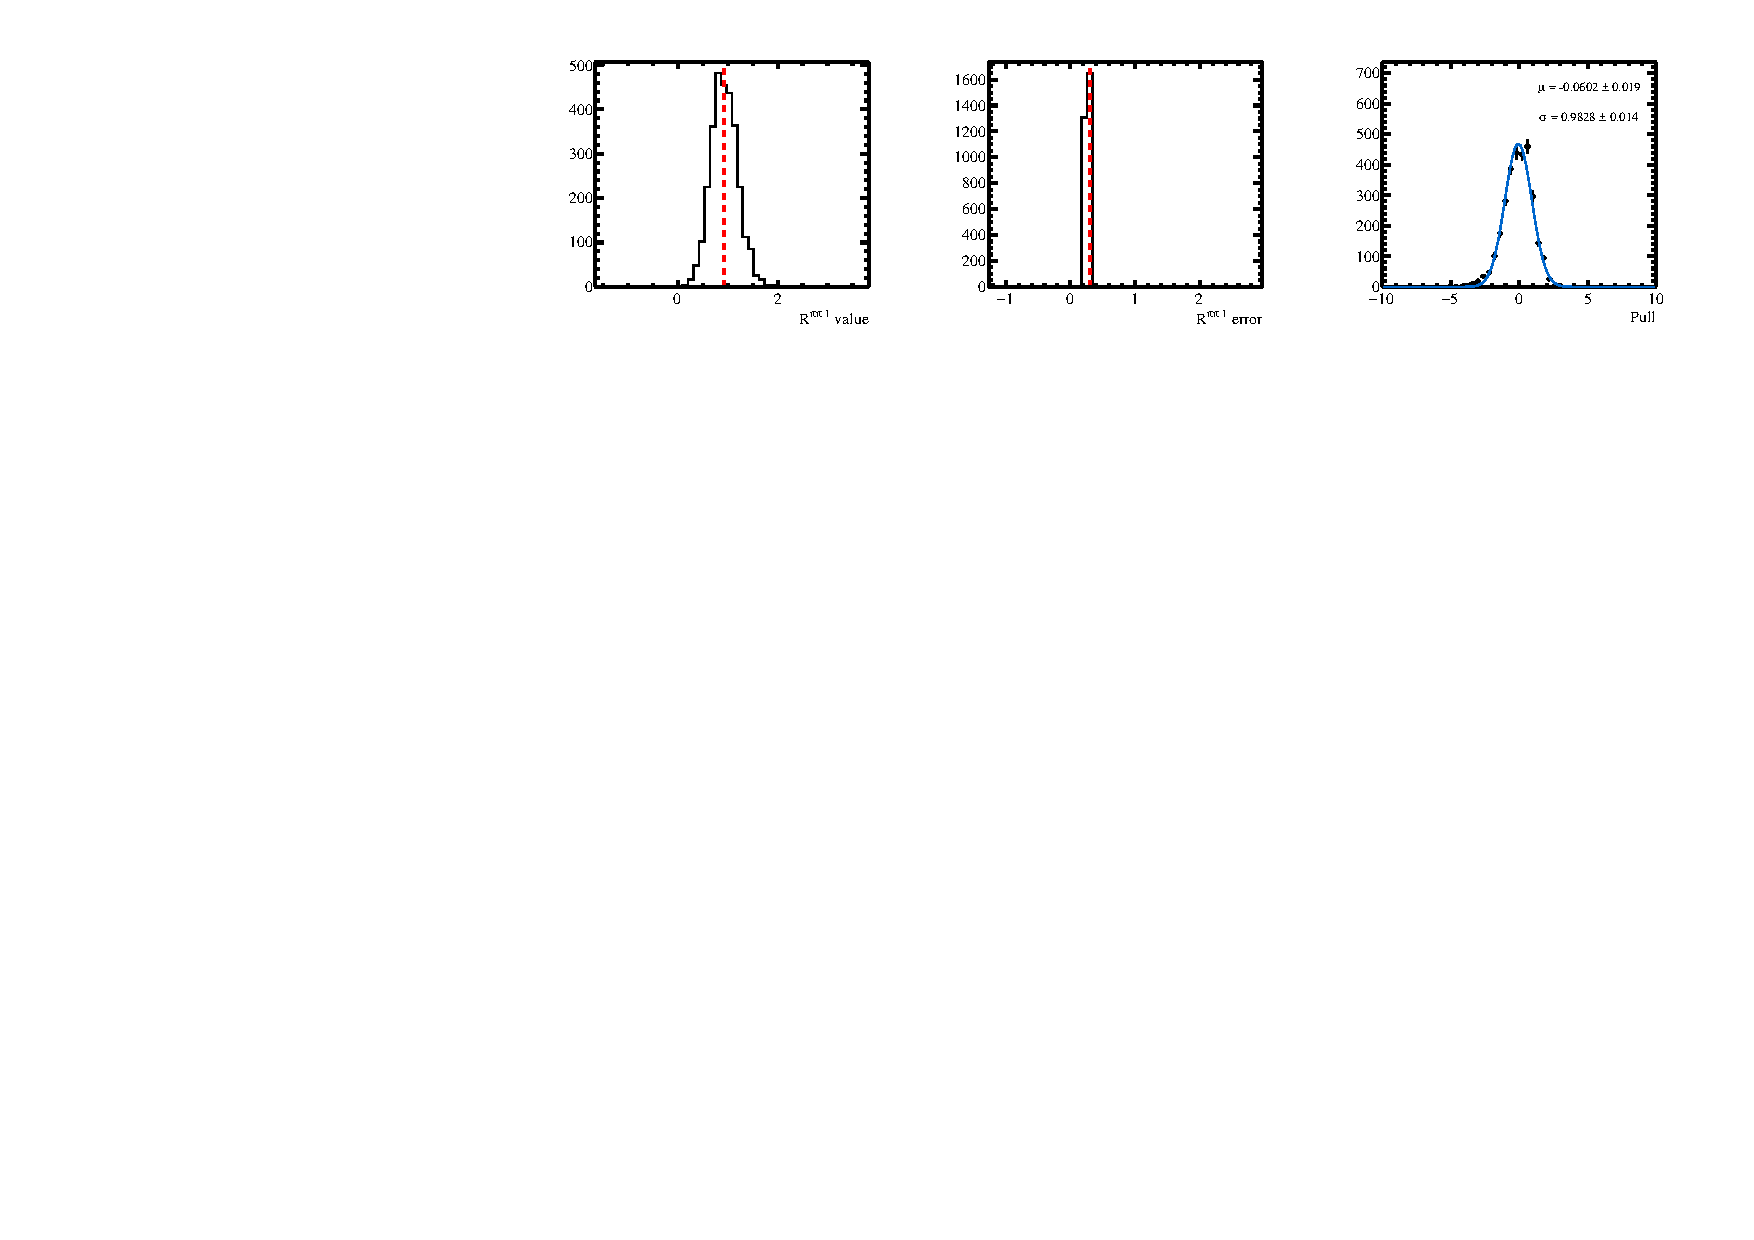
\includegraphics[width=0.7\textwidth]{ANA_resources/Plots/Data_fit/FitterBias//R_signal_pipi_run1.pdf} \\
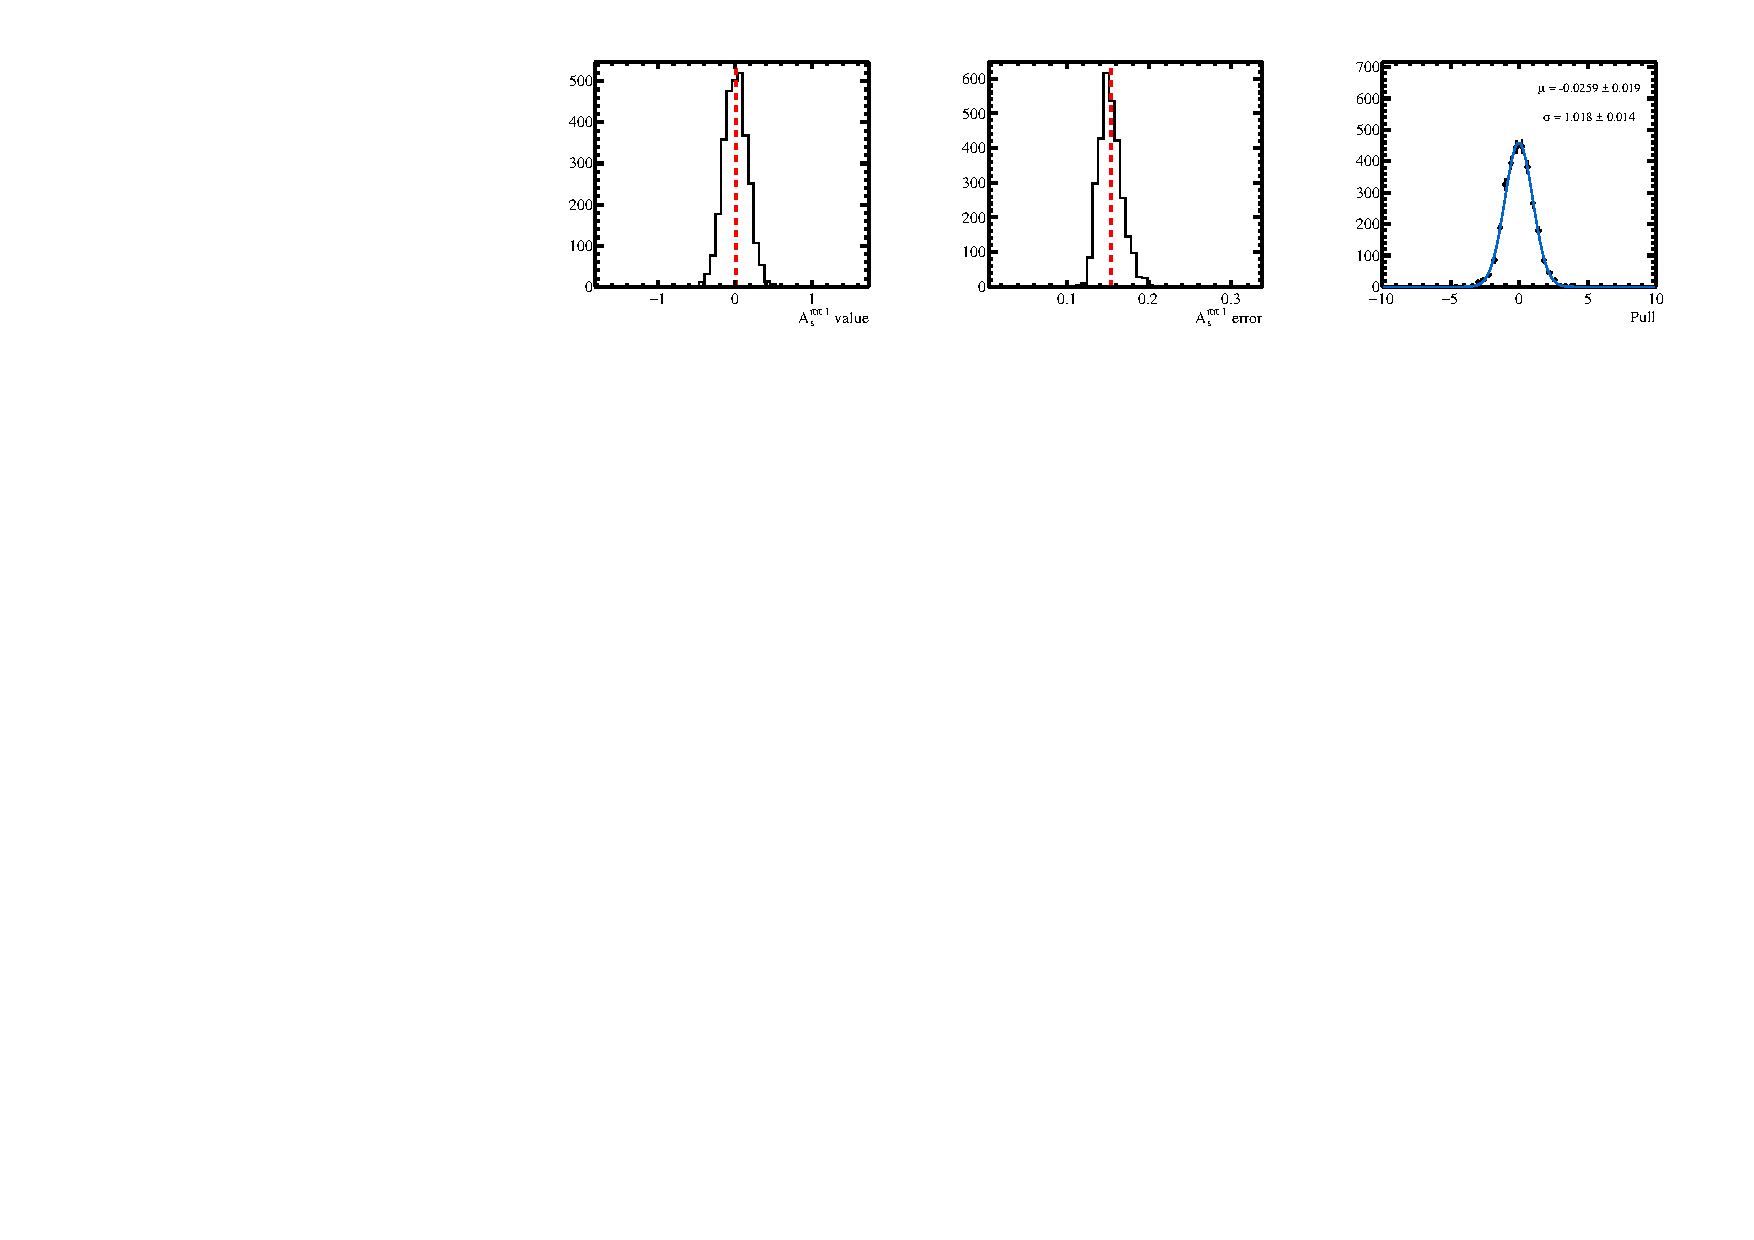
\includegraphics[width=0.7\textwidth]{ANA_resources/Plots/Data_fit/FitterBias//A_Bs_pipi_run1.pdf} \\
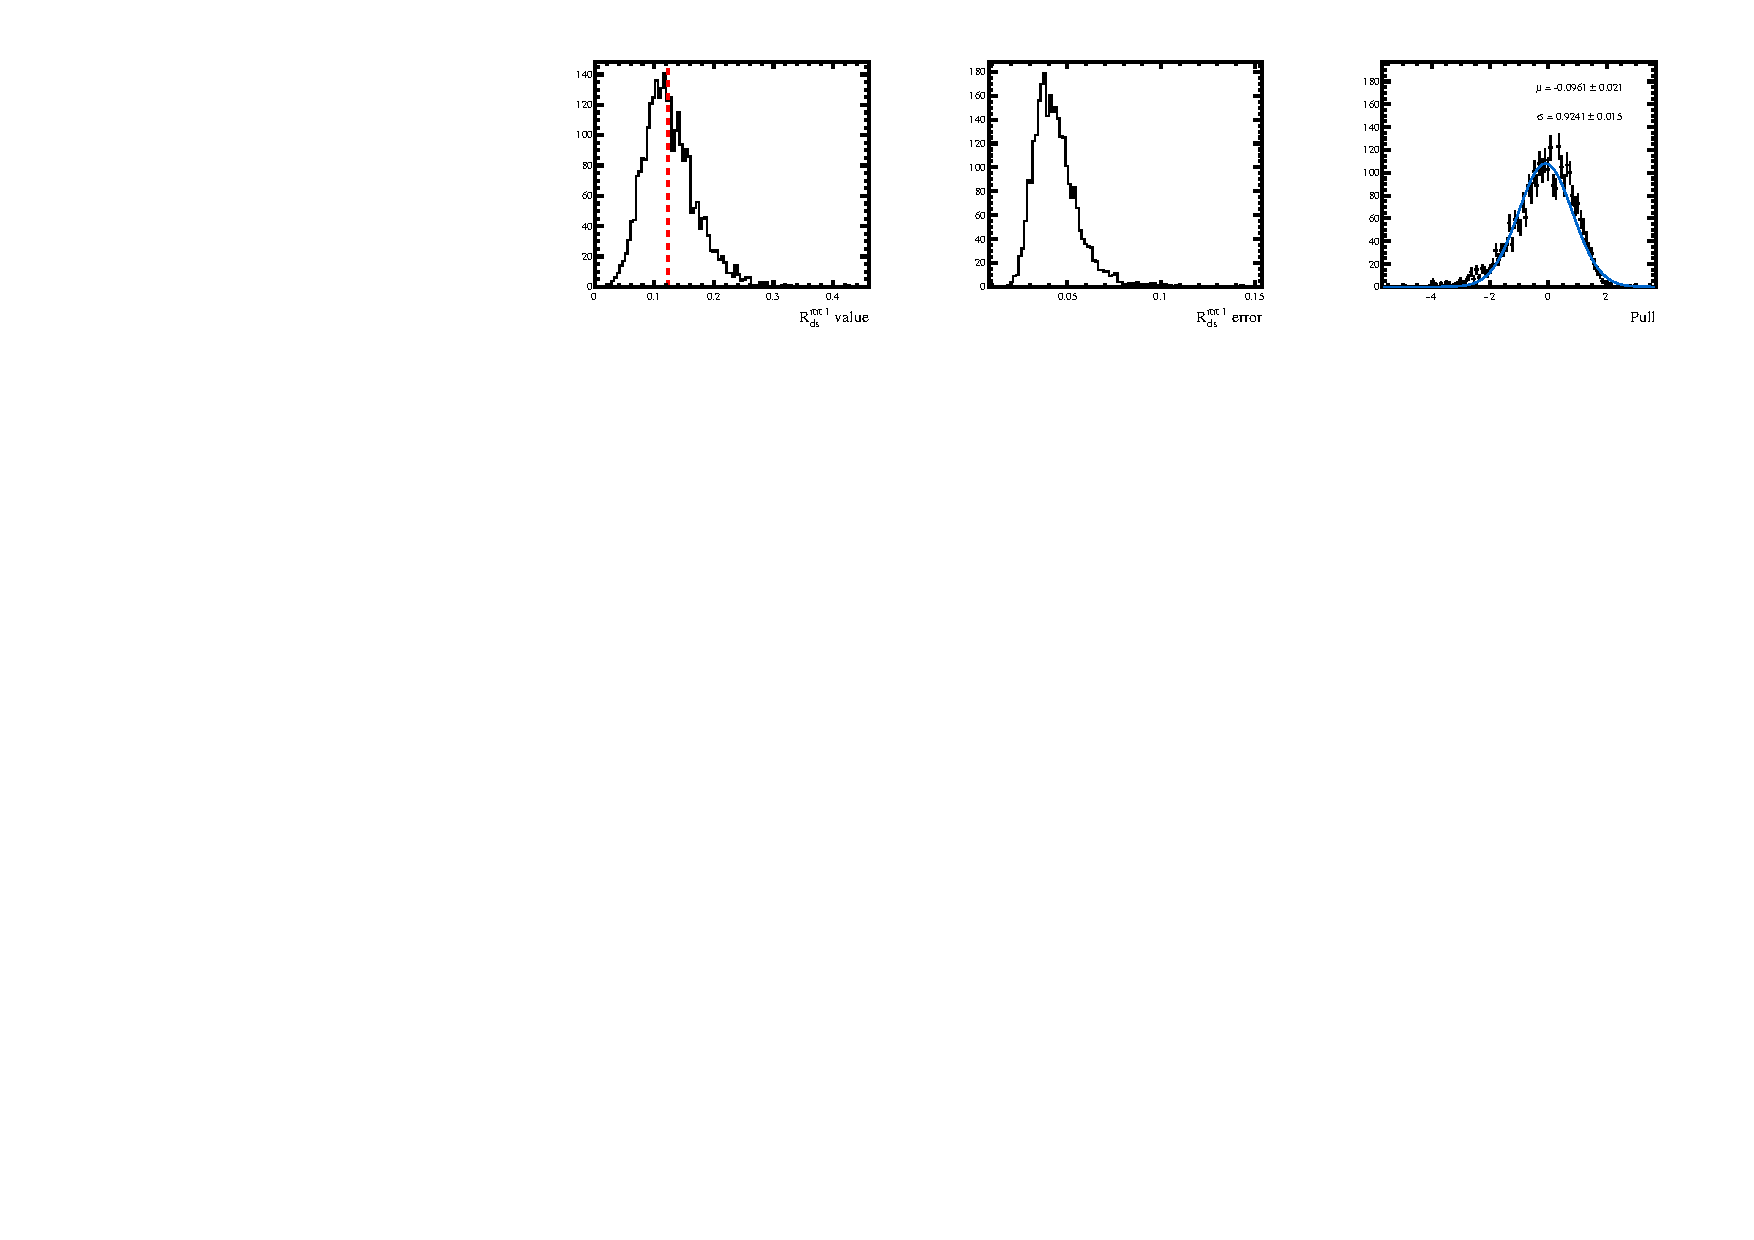
\includegraphics[width=0.7\textwidth]{ANA_resources/Plots/Data_fit/FitterBias//R_ds_pipi_run1.pdf} \\
  \end{tabular}
  \caption{Pull plots for Run 1 GLW parameters of interest, obtained from generating and fitting 1000 toys using the data fit model. The left hand plot shows the fitted parameter distribution, with the value used to generate the parameter indicated with a dotted red line. The central plot shows the fit error, and the right hand plot shows the pull distribution fitted with a Gaussian.}
\label{fig:GLW_run1_pulls}
\end{figure}
